\chapter{Dimostrazione di proprietà di funzioni}

\qs{}{Date una funzione e una specifica di ciò che la funzione dovrebbe calcolare, la funzione è corretta rispetto alla specifica?}

\qs{}{Date due funzioni (una corretta ma inefficiente e una efficiente ma più complessa da capire), sono equivalenti?}

\paragraph{Test:}

\begin{itemize}
    \item facile (soprattutto se il linguaggio non è imperativo);
    \item non è esaustivo (possono esserci casi non considerati).
\end{itemize}

\paragraph{Dimostrazione:}

\begin{itemize}
    \item difficile (soprattutto se il linguaggio è imperativo);
    \item è esaustiva.
\end{itemize}

\section{Dimostrazioni su numeri interi}

\begin{lstlisting}
foo :: Int -> Int -> Int -> Int
foo x y z | y < x       = foo y x z
          | z < y       = foo x z y
          | otherwise   = z
\end{lstlisting}

\qs{}{$\forall\:\: x,\:\:y,\:\:z = \text{max }\{x,\:\:y,\:\:z\}$ è una proprietà vera?}

Si possono fare dei test, ma saranno sempre in numero finito. Per cui è più conveniente cercare una dimostrazione.

\subsection{Dimostrazione per casi}

\nt{I numeri sono infinite, per cui non si può verificare il comportamento per ogni combinazione. Ma l'ordine tra i numeri è totale, per cui possiamo considerare un numero finito di casi che è esaustivo}

\begin{center}
    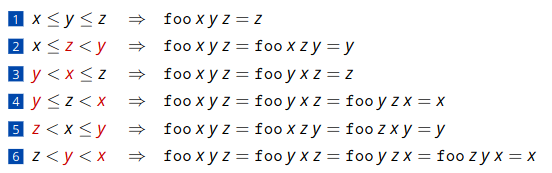
\includegraphics[scale = 0.7]{images/funzioni/Casi.png}    
\end{center}

\nt{Il codice è tutto ciò che serve per ragionare sui casi}

\subsection{Induzione}

\nt{L'approccio precedente è attuabile solo se il numero dei casi da prendere in considerazione è finito. Il principio di induzione permette di dimostrare una proprietà su un insieme infinito di casi}

\dfn{Il principio di induzione}{Data una proprietà $P(n)$ dei numeri naturali, se:
\begin{itemize}
    \item $P(0)$;
    \item $P(n)$ implica $P(n + 1)$ per ogni $n \in \bbN$.
\end{itemize}
allora $P(n)$ per ogni $n \in \bbN$
}
\begin{lstlisting}
exp :: Int -> Int -> Int -> Int
exp _ 0 = 1
exp x n = x * exp x (n - 1)
\end{lstlisting}
\ex{Esponenziale}{

Si vuole dimostrare che:
\begin{enumerate}
    \item $\forall\:\:x,\:\:m \geq 0,\:\:n\geq 0 : \text{exp } x\:\:(m + n) = \text{exp } x\:\:m * \text{exp} x |:\: n$;
    \item $\forall \:\:x, \:\:n : \text{exp }(x * x)\:\:n = \text{exp } x\:\:n * \text{exp } x\:\:n$.
\end{enumerate}
\pagebreak
\paragraph{Prima dimostrazione:}
\begin{center}
    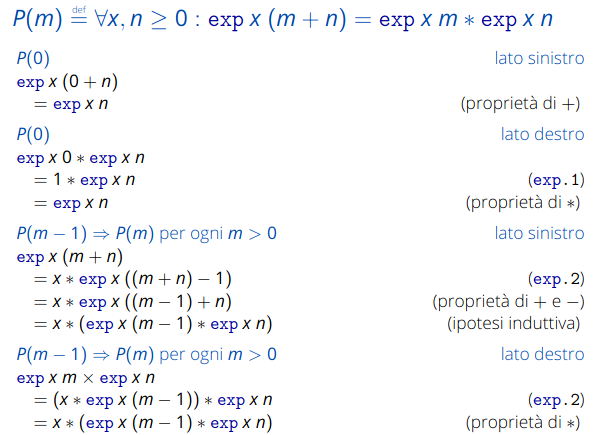
\includegraphics[scale = 0.7]{images/funzioni/Dim1.png}    
\end{center}
\paragraph{Seconda dimostrazione:}
\begin{center}
    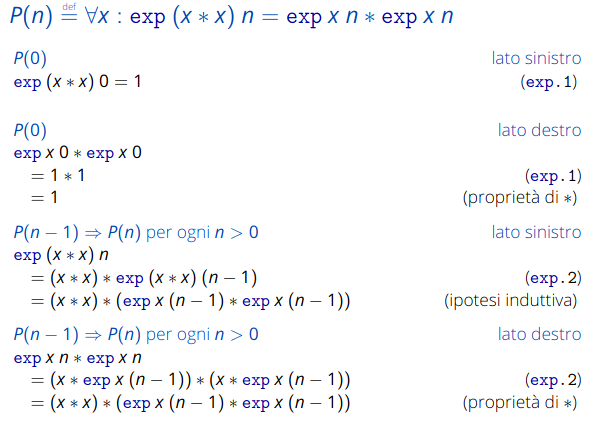
\includegraphics[scale = 0.7]{images/funzioni/Dim2.png}    
\end{center}
}

\dfn{Principio di induzione forte}{Data una proprietà $P(n)$ dei numeri naturali, se:
\begin{itemize}
    \item $(\forall \:\: m < n : P(m))\Rightarrow P(n)$, per ogni $n \in \bbN$.
\end{itemize}
allora $P(n)$ per ogni $n \in \bbN$
}

\nt{Il principio di induzione forte è equivalente al principio di induzione}

\section{Dimostrazioni sulle liste}

\dfn{Principio di induzione sulle liste finite}{
Data una proprietà $P(xs)$ delle liste, se:
\begin{itemize}
    \item $P([])$;
    \item $P(xs)$ implica $P(x\:\: :\:\:xs)$ per ogni $x$ e $xs$.
\end{itemize}
Allora $P(xs)$ per ogni lista finita $xs$.
}

\ex{Length}{
\begin{center}
    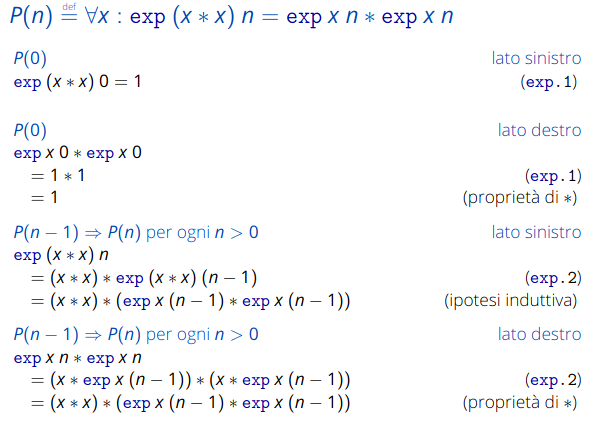
\includegraphics[scale = 0.7]{images/funzioni/Dim2.png}    
\end{center}
}
\nt{Può capitare, durante una dimostrazione, di osservare passaggi intuitivi di cui non si ha una prova. Per cui si possono assumere e poi dimostrare in seguito}

\section{Dimostrazioni sugli alberi}

\dfn{Principio di induzione sugli alberi}{
Data una proprietà $P(t)$, se:
\begin{itemize}
    \item $P(Leaf)$;
    \item $P(t_1) \wedge P(t_2)$ implica $P(Branch\:\:t_1 t_2)$ per ogni $x$, $t_1$ e $t_2$.
\end{itemize}
Allora  $P(t)$ per ogni albero (finito) $t$.
}

\ex{Trees}{
    \begin{center}
        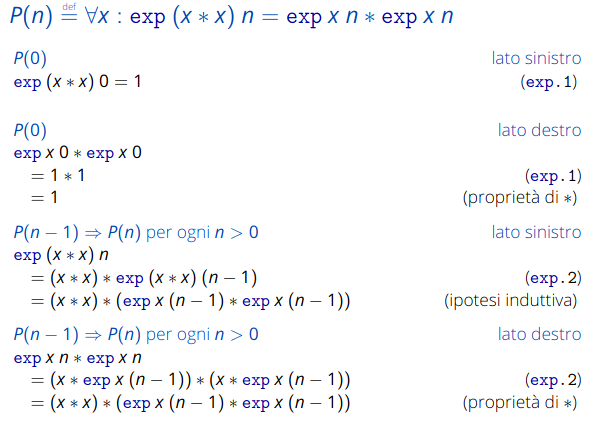
\includegraphics[scale = 0.7]{images/funzioni/Dim2.png}    
    \end{center}
}

\section{Dimostrazioni sulle funzioni di ordine superiore}

\dfn{Principio di estensionabilità}{
Due funzioni $f$ e $g$ sono uguali se producono lo stesso risultato
quando sono applicate allo stesso argomento. Formalmente:
$$(\forall x\: :\: f\: g = g\: x) \Leftrightarrow f = g$$
}

\nt{
È il principio che giustifica la regola di $\eta$-riduzione.    
}

\cor{proprietà della composizione funzionale}{
    \begin{center}
        \includegraphics[scale = 0.7]{images/funzioni/Proprietà.png}    
    \end{center}
}

\thm{Legge di fusione}{
Se:
\begin{itemize}
    \item $f\:a = b$;
    \item $f\:(g\:x\:y) = h\:x\:(f\:y)$;
\end{itemize}
allora
\begin{itemize}
    \item $f\:.\:\text{foldr}\:g\:a = \text{foldr}\:h\:b$.
\end{itemize}
}

